\section{Espectro de energía}
\justifying

\subsection{Niveles de Landau}
\begin{frame}{Niveles de Landau}
	\begin{multicols}{2}
	\scriptsize{En presencia de un campo magn\'etico, los electrones solo pueden ocupar \'orbitas con estados discretos de energ\'ia, llamados niveles de Landau (L.L. Por sus siglas en ingl\'es).	Estos niveles vienen dados por la ecuaci\'on:
	\begin{equation}
		E_n = \hbar \omega_c (n+\frac{1}{2})
		\label{eq:landau}
	\end{equation}
	donde $\hbar$ es la constante de planck normalizada, $n\in \mathbb{Z}$ y  $\omega_c=\frac{eB}{mc}$ es la frecuencia del ciclotrón,
	$e$ es la carga del electrón, $B$ la magnitud del campo magnético, $m$ la masa y $c$ es la velocidad de la luz.}
	\begin{figure}[b!]
		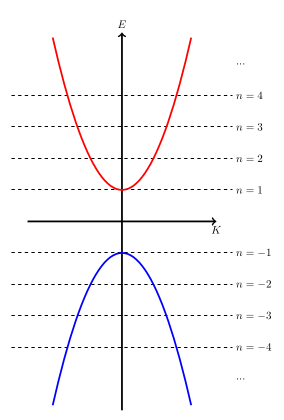
\includegraphics[width=3cm,height=4.5cm]{graficas/LL_material.png}
			\caption{\scriptsize{Niveles de Landau en material convencional}}
	\end{figure}
	\end{multicols}
\end{frame}

\begin{frame}{Niveles de Landau en el grafeno}
	\begin{multicols}{2}
		\scriptsize{En el grafeno, los niveles de Landau se pueden obtener a partir de considerar el hamiltoniano,
						$\hat{H}=\frac{\hat{\pi}^2}{2m}+V(\vec{r})$ siendo $\hat{\pi}=\vec{p}- \frac{e}{c}\vec{A}$
						y $\vec{A}$ es el potencial vector, de la forma:
			\begin{equation}
					\hat{H} = \sqrt{\frac{2e\hbar B \nu_f}{c}}
					\left( \begin{array}{c c}
							0&\hat{a}\\
							\hat{a}^\dagger&0
					\end{array} \right)
			\end{equation}
			donde $\hat{a}= \sqrt{c/2e\hbar B}(\pi_x-i\pi_y)$ y 	$\hat{a}^\dagger=\sqrt{c/2e\hbar B}(\pi_x+i\pi_y)$.\\
			Resolviendo la ecuación de Schrödinger se obtiene:
			\begin{equation}
					E_n= \pm \hbar\omega_c \sqrt{n}
			\end{equation}
			donde $\omega_c = \sqrt{2}\nu_f/l_B$ es el ciclotrón cuántico y $l_B = \sqrt{\frac{\hbar c}{e B}}$ es la longitud magnética.}
		\begin{figure}
			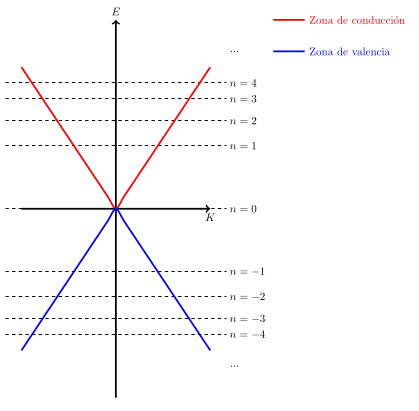
\includegraphics[height=4cm]{graficas/LL_grafeno.png}
			\caption{\scriptsize{Niveles de Landau en el grafeno}}
		\end{figure}
	\end{multicols}
\end{frame}

\begin{frame}{Degenerancia de los niveles de Landau}
	Considerando el movimiento de un electrón libre en un campo magnético externo constante,
	el hamiltoniano adquiere la forma:
	\begin{equation}
		\hat{H} = \frac{1}{2m}\left( \vec{p}-\frac{e}{c}\vec{A} \right)^2
		\label{hamil_nr}
	\end{equation}

	con lo que la ecuación de Schrödinger queda de la siguiente manera:

	\begin{equation}
			-\frac{\hbar^2}{2m}\frac{\partial^2\psi}{\partial x^2} + \frac{1}{2m} \left( -i\hbar \frac{\partial}{\partial y} -\frac{e}{c}Bx \right)^2 \psi - \frac{\hbar^2}{2m} \frac{\partial^2\psi}{\partial z^2} = \varepsilon \psi
			\label{sch_nr}
	\end{equation}
\end{frame}

\begin{frame}
	Proponiendo una solución $\psi(x,y,z) = e^{\frac{i}{\hbar}(p_yy+p_zz)}\psi(x),$
	y sustituyendo en la ecuación (\ref{sch_nr}), se obtiene:

	\begin{equation}
    -\frac{\hbar^2}{2m}\frac{\partial^2\psi(x)}{\partial x^2} + \frac{1}{2m} \left( p_y-\frac{e}{c}Bx \right)^2 \psi(x) + \frac{p_z^2}{2m} \psi(x) = \varepsilon \psi
	\end{equation}
	\begin{equation}
    -\frac{\hbar^2}{2m}\frac{\partial^2\psi(x)}{\partial x^2} + \frac{e^2B^2}{2mc^2} \left( x-\frac{p_yc}{eB} \right)^2 \psi(x)  = \left(\varepsilon -\frac{p_z^2}{2m}\right) \psi
    \label{sch_nr2}
	\end{equation}
\end{frame}

\begin{frame}
	La ecuación \ref{sch_nr2} es similar a la de un oscilador armónico.\\
	Al comparar, se tiene que
	\begin{equation}
    \varepsilon = \frac{p_z^2}{2m} + \frac{e\hbar B}{mc}\left(n+\frac{1}{2}\right)
	\end{equation}
	donde la cantidad $\frac{eB}{mc}$ juega papel de $\omega$  y $\varepsilon -\frac{p_z^2}{2m}$ es la energía del oscilador.
\end{frame}

\subsection{Estados de Bloch en grafeno en un campo eléctrico}

\begin{frame}{Estados de Bloch en el grafeno}
	Para un sistema sustrato-grafeno, el hamiltoniano se puede escribir de la forma:
	\begin{equation}
			\hat{H} = \hat{\vec{p}}+\frac{e}{c}\hat{\vec{A}} + \hat{U},
	\end{equation}

	\begin{figure}[t]
		\centering
		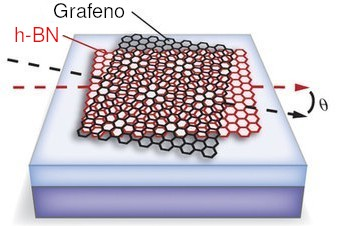
\includegraphics[scale=0.4]{graficas/Moire.jpg}
		\caption{Patrón de Moiré en una capa de grafeno sobre hBN.}
		\label{moire}
	\end{figure}
\end{frame}

\begin{frame}
	donde $\hat{U}(x,y)$ puede ser aproximado por la expresión \cite{Wang2004}:
	\begin{equation}
			\hat{U}(x,y)=U_{x}\cos (K_{x}x)\cos (K_{y}y)+\frac{U_{y}}{2}\left[ 1+\cos (2K_{y}y)\right],
	\end{equation}
	siendo
	\begin{equation}
		K_{x}=\frac{2\pi}{a_{x}},\hspace{1cm}K_{y}=\frac{2\pi}{\sqrt{3}a_{y}},
	\end{equation}
	donde $a_x$ y $a_y$ son los periodos de la celda elemental.
\end{frame}

\begin{frame}
	El espectro de energía está dado por la expresión \cite{Wang2004}:
	\begin{equation}
			\epsilon = \pm \epsilon_n + \zeta(k_x,k_y),
	\end{equation}
	donde $\epsilon_n = \hbar\omega_f\sqrt n $ y
	$\zeta(k_x,k_y)$ es la energía asociada a la estructura de estados de Bloch.
	Por lo tanto, las bandas de Landau se dividen en subbandas,
	lo que lleva a una ampliación del espectro magnético.
\end{frame}

\begin{frame}
	Dicha energía puede expresarse de la siguiente manera \cite{Wang2004}:
	\begin{equation}
			\zeta(k_{y}, \beta)=\frac{U_{y}}{2}\left[1+F_{n}(4u_{y})\cos 2\beta\right]+U_{x}F_{n}(4u_{y})\cos \gamma\cos \beta,
	\end{equation}
	donde
	\begin{equation}
		F_{n} (4u_{y}) = e^{- u_{y} / 2} \left[L_{n} (4u_{y}) + L_{n-1} (4u_{y}) \right],
	\end{equation}

	$L_n$ son los polinomios de Laguerre y $ u_{y} = l^{2} K_{y}^{2} / 2 $
\end{frame}

\begin{frame}
	\begin{equation}
		\gamma = K_{x} l^{2} (k_{y} + K_{y}) 2,\hspace{1cm} \beta = l^{2} K_{y} k_{x }
	\end{equation}

	Las componentes $ k_{y} $ y $ \beta $ se definen dentro de los intervalos
	\begin{equation}
	-a_{x} / 2l^{2} \leq k_{y} \leq a_{x} / 2l^{ 2},\hspace{1cm}0 \leq \beta \leq 2 \pi.                                                                               \end{equation}

  El ancho de las bandas de Landau está modulado por los polinomios de Laguerre $L_n$,
	los cuales son funciones oscilantes de la razón $\Phi_o/\Phi$.
\end{frame}
